\documentclass[final]{beamer}

\mode<presentation>
{
  \usetheme{CPC}
}

% additional settings
\setbeamerfont{itemize}{size=\normalsize}
\setbeamerfont{itemize/enumerate body}{size=\normalsize}
\setbeamerfont{itemize/enumerate subbody}{size=\normalsize}

\usepackage{lmodern}

% additional packages
\usepackage{amsmath,amsthm, amssymb, latexsym}
\usepackage[english]{babel}
\usepackage[utf8]{inputenc}
\usepackage[orientation=landscape,size=a0,scale=2]{beamerposter}

\usepackage{microtype}
\usepackage{color}
\usepackage{fancyvrb}

\usepackage{color}
\usepackage{listings}
\usepackage{bm}
\usepackage{calc}

\newcommand{\neghalfthinspace}{\kern -0.0833em}

\lstset{ %
  basicstyle=\ttfamily\small,  %
  breaklines=true, %
  keywordstyle=\textbf %
}

\title{User guided outlier detection in heterogeneous datasets}
\author{Clément Pit-\kern0pt-Claudel, Zelda Mariet, Rachael Harding}
\institute[MIT]{Massachusetts Institute of Technology}
\date{Dec. 10, 2014}

\newlength{\colwidth}
\newlength{\doublecolwidth}
\newlength{\blocksep}

\begin{document}
\begin{frame}[fragile]{}
  \setlength{\blocksep}{1.5ex}
  \setlength{\colwidth}{(\linewidth - 2\blocksep)/3}
  \setlength{\doublecolwidth}{2\colwidth + \blocksep}

  \begin{columns}[T]
    \begin{column}{\colwidth}
      \begin{block}{\thighlight{Motivation}}
  \begin{itemize}
  \item \highlight{Highlighted word}. BLAH BLAH
  \item 
  \item 
  \item 
  \end{itemize}
\end{block}
 \vspace{\blocksep}
      
\newcommand{\edgeb}{yellow}
\newcommand{\fillb}{red}
\newcommand{\textb}{blue}
\begin{block}{\thighlight{Example: Outliers in the CSAIL directory}}
\vspace{-1cm}
\begin{table}
\begin{tabular*}{\colwidth - \blocksep}{c|c|c|c}
LastName & FirstName & Office & Email\\
\hline
Harding&Rachael&\fcolorbox{\edgeb}{\fillb}{\color{\textb}\textbf{32-888}}&rhardin@mit.edu\\
Mariet&Zelda&32-G414&mariet@mit.edu\\
\fcolorbox{\edgeb}{\fillb}{\color{\textb}\textbf{Pit--claudel}}&Clement&32-G804&cpitcla@mit.edu\\
\end{tabular*}
\end{table}
\vspace{-1cm}

\end{block}
 \vspace{\blocksep}
      \begin{block}{\thighlight{Our Approach}}
  \subttl{Tuple expansion}
  \begin{itemize}
  	\item \texttt{"32-G414"~} $\longrightarrow
  	  \begin{cases}
  	  	\text{length: } & \texttt{7}\\
  	  	\text{pattern: } & \texttt{NNPLNNN}\\
  	  	\text{uppercase: } & \texttt{True (1)}\\
  	  	\ldots
  	  \end{cases}$
  	  
    	\item \texttt{1418178600} $\longrightarrow
  	  \begin{cases}
    	  	\text{date: } & \texttt{(2014,12,10)}\\
    	  	\text{dow: } & \texttt{Wed (2)}\\
    	  	\text{binary: } & \texttt{0b101...0010}\\
    	  	\ldots
  	  \end{cases}$
  \end{itemize}
  
  
  \subttl{3 pass pipeline}
	\begin{itemize}
		\item Statistical analysis
		\item Data modeling
		\item Outlier detection
	\end{itemize}
\end{block}


    \end{column}
    
    \begin{column}{\doublecolwidth}
      \begin{block}{\thighlight{Our pipeline}}
        \begin{figure}
          \centering
          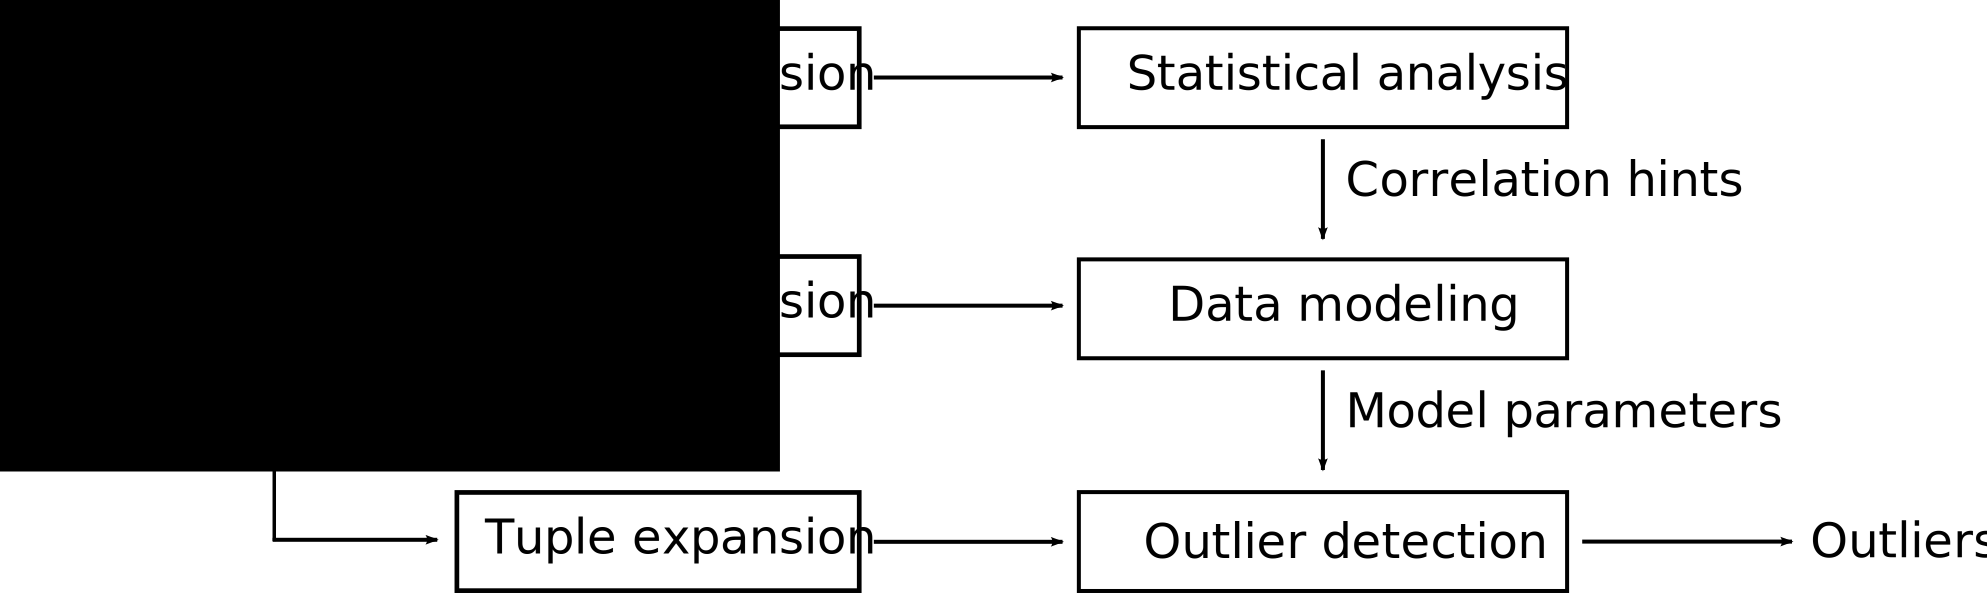
\includegraphics[width=\linewidth]{../graphics/pipeline.pdf}
        \end{figure}
      \end{block} \vspace{\blocksep}

      \vspace{-\baselineskip}
      \begin{columns}[t,totalwidth=\textwidth] % 
        \begin{column}{\colwidth}
          \begin{block}{\thighlight{Outlier characterization and detection}}
\end{block}
 \vspace{\blocksep}
        \end{column}

        \begin{column}{\colwidth}
          \section{Evaluation}
\label{sec:evaluation}

We implemented dBoost in approximately 2000 lines of \texttt{python3} code. Our code is publicly available on GitHub under version 3 of the GNU Public License~\footnote{\url{https://github.com/cpitclaudel/6.830}}. The program is made of two parts: a library, and a number of data acquisition front-ends (CSV and SQL are currently supported). The library provides functions for each of the phases previously described.

Table~\ref{table:flags} shows the usage options to run the models supported by dBoost. \fxnote{Should we keep this table?}

\begin{table*}
  \renewcommand{\arraystretch}{1.2}
  \setlength\tabcolsep{3\tabcolsep}

  \label{table:flags}
  \caption{dBoost command line usage.}
  \centering
  \begin{tabular} { l | l | p{10cm} }
    \multicolumn{3}{l}{} \\
    \hline
    Flag & Options & Explanation \\
    \hline
    --gaussian & n\_stdev & Report outliers that fall more than n\_stdev standard deviations away from the mean of the data \\
    --mixture & n\_subpops & Use a model of \texttt{n\_subpops} Gaussians \\
         & threshold & Report outliers above threshold percentile \\
    --histogram & peak\_s & Consider only fields with a peaked distribution with peakiness peak\_s \\
         & outlier\_s & Report values that fall in classes with less than outlier\_s percent \\
    --statistical & epsilon & Give hints to the model for correlations with Pearson $R$ coefficient greater than epsilon \\
  \end{tabular}
\end{table*}

This sections presents the results of running our tool on a mix of real and synthetic datasets.

To evaluate of our tool, we used a mix of synthetic and real datasets, succinctly described below:

\begin{itemize}
\item \emph{Synthetic datasets}
  \begin{description}
  \item[Fizz-Buzz] A mixed textual-numerical dataset in which each record contains two entries: a number, and either ``Fizz'' if the number is divisible by 3, ``Buzz'' if the number is divisible by 5, ``FizzBuzz'' if it is divisible by both, and the number itself (as a string) otherwise. Outliers appear when the second column does not respect these rules; this can be a misplaced ``Fizz'', a missing ``Buzz'', or even a totally different string (e.g. ``Woof'').
  \item[Web logins] A series of three non-numeric datasets in which entries record the time and place of connection for different users. Each user has different connection habits, leading to different types of outliers.
  \item[TODO] Continuous dataset
  \end{description}
\item \emph{Real-world datasets}
  \begin{description}
  \item[CSAIL Directory] A publicly-accessible directory of researchers\fxnote{Should we anonymize this?}, in which each record include a first and a last name, a phone number, an office number, an email, and a job title. Outliers are hard to define mathematically in this case, and we instead demonstrate how the ideas exposed in previous sections of the paper come together to allow for efficient detection of unwanted values.
  \item[Intel lab data] A publicly-available numeric dataset of temperature, light, and humidity measurements. Outliers are due mostly to sensor glitches.
  \end{description}
\end{itemize}

These datasets showcase the power of our methods, both in terms of classification power, and in terms of expressiveness and succinctness when adding new rules to the system\footnote{Indeed, the set of rules used for tuple expansion is user-configurable, and new rules can be easily added; thus, specific knowledge about the data can be taught to the system by users, expressing some soft form of data integrity constraints.}.

The following subsections describe each of the test sets and associated results in greater detail.

\subsubsection{Soft constraint specifications: Fizz-Buzz}
The Fizz-Buzz programming exercise is based on a children's game and frequently found in programming interviews. The synthetic dataset we generated obeys the following rules: for each record <x, y>, $x$ is a number between 0 and 1000, and $y$ is ``Fizz'' if \(x \mod 3 = 0\), ``Buzz'' if \(x \mod 5 = 0\), ``FizzBuzz'' if \(x \mod 15 == 0\), and \(x\) otherwise. However, we introduced three outliers to this data: \texttt{(25, "Fizz")}, \texttt{(28, "Woof!")}, \texttt{(30, "Buzz")}. Each demonstrates a different error, namely swapping \texttt{"Fizz"} and \texttt{"Buzz"}, producing entirely incorrect output, and failing to recognize that a number is divisible by both $3$ and $5$.

A traditional way of checking that all tuples verify the production rule outlined above is to encode this rule itself as a database integrity constraint. This requires encoding the full complexity of the exercise in the rule. If the exercise were to change, new cases must be added manually. Instead, a user might want to specify the bare minimum for the system to infer the rules; in this case, it is sufficient to add one extraction rule, mapping integers to two booleans denoting whether they are divisible by $3$ or $5$. Such a rule could be written like this:

\begin{minted}{python3}
@rule
def fizzbuzz(x: int) -> ("div 3", "div 5"):
  return (x % 3 == 0, x % 5 == 0)
\end{minted}

Running the discrete statistical analyzer on the synthetic datasets suggests that the two columns are correlated, and using the histogram model flags the aforementioned outliers. The output of the program for the \texttt{(30, "Buzz")} line, for example, is similar to:

\begin{lstnobreak}[gobble=2]
   $30$ $Buzz$
   > Values ($30$, $'Buzz'$) (0, 1) do not match
     features ($'div 3'$, $'erase numbers'$)
     • histogram for ('div 3', 'erase numbers'):
       █████ (False, 'Buzz')
       (False, 'Fizz')
       (False, 'Woof!')
       ██████████████████ (False, '<num>')
       $(True, 'Buzz')$
       ██████████ (True, 'Fizz')
       ██ (True, 'FizzBuzz')
\end{lstnobreak}

Using the partitioned histogram model produces similar output:

\begin{lstnobreak}[gobble=2]
   $30$ $Buzz$
   > Values ($30$, $'Buzz'$) (0, 1) do not match
     features ($'div 3'$, $'strp'$)
     • histogram for ('strp',) if 'div 3' = True:
       $('Buzz',)$
       ████████████████████ ('Fizz',)
       ████ ('FizzBuzz',)
     ... if 'div 3' = False:
       ████████████████████ ('<num>',)
       █████ ('Buzz',)
       ('Fizz',)
       ('Woof!',)
\end{lstnobreak}

\input{logins-evaluation}
\subsection{CSAIL Directory}
\label{sec:csail-directory-evaluation}

The CSAIL directory is an online directory of about 1000 faculty, staff and students in the MIT Computer Science and Artificial Intelligence Laboratory\footnote{\url{https://www.csail.mit.edu/peoplesearch}}. Each entry contains a person's name, phone number, office number, email address, and position.

Some data, such as a phone number, may be missing from the directory. Still, we expect our framework to be useful in flagging discrepancies between different records. Since the notion of what constitutes an outlier here is imprecise at best, we also expect the tool to allow the user to explore different sets of parameters. To illustrate the process, we dicuss the results returned by three distinct iterations of the tool in the next section, each with increasingly strict limits on the number of outliers returned. Because the CSAIL test set is exclusively textual, we use the histogram model for evaluation.

\subsubsection{Initial run: low specificity filtering}
The search for outliers is initiated with parameters $\theta = 0.8, \epsilon = 0.2$. Correlation detection is disabled for these experiments.

This invocation produces a long list of outliers; a small subset of these is presented below. For privacy reasons, names,  phone numbers, office numbers, and emails have been omitted or anonymized in the following listings.

\begin{lstlisting}[gobble=2]
  Hacker, Alyssa, 32-D968,
    $aph@CSAIL.MIT.EDU$, Postdoctoral Associate

  Bitdiddle, Ben, $32-221B$,
    bbitdid@csail.mit.edu, Graduate Student

  $Lu-ater$, Eva, 32-G972,
    eva@csail.mit.edu, Research Scientist
\end{lstlisting}

In total, 451 entries contain outliers, out of a total of 1000. Office numbers are often flagged, as well as names and email addresses. By changing the input parameters to $\theta = 0.8, \epsilon = 0.2$, most of the outliers due to office numbers disappear due to the lower sensitivity. \lstinline{Hacker, Alyssa} disappears from the list, since e-mails with the domain in all capitalization occur frequently enough in the database that they are not considered outliers at sensitivity level $\epsilon = 0.05$. In total there are $68$ outliers.


%\begin{lstlisting}[gobble=2]
%  Bitdiddle, Ben, $32-221B$,
%    bbitdid@csail.mit.edu, Graduate Student
%  > Value $'32-221B'$ (3) doesn't match
%    feature $'signature'$
%
%  $Lu-ater$, Eva, 32-G972,
%    eva@csail.mit.edu, Research Scientist
%  > Value $'Lu-ater'$ (1) doesn't match
%    feature $'title case'$
%\end{lstlisting}


In addition to identifying outliers, dBoost is equipped with tools that provide the user with additional feedback on why features were identified as outliers.

\begin{lstlisting}[gobble=2]
  Bitdiddle, Ben, $32-221B$,
    bbitdid@csail.mit.edu, Graduate Student
  > Value $'32-221B'$ (3) doesn't match
    feature $'signature'$
  • histogram for ($'signature'$,):
    ██████████
    Lu,Lu,Nd,Nd,Pd,Nd,Nd,Nd
    Lu,Nd,Nd,Pd,Nd,Nd,Nd
    Nd,Nd,Lu,Pd,Nd,Nd,Nd
    ████████████████████ Nd,Nd,Pd,Lu,Nd,Nd,Nd
    ██ Nd,Nd,Pd,Lu,Nd,Nd,Nd,Lu
    ██████ Nd,Nd,Pd,Nd,Nd,Nd
    $█ Nd,Nd,Pd,Nd,Nd,Nd,Lu$
    Nd,Nd,Pd,Nd,Nd,Nd,Nd
    Nd,Pd,Nd,Nd,Nd

  $Lu-ater$, Eva, 32-G972,
    eva@csail.mit.edu, Research Scientist
  > Value $'Lu-ater'$ (1) doesn't match
    feature $'title case'$
  • histogram for ($'title case'$,):
    $False$
    ████████████████████ True
\end{lstlisting}

Our tool highlights the incorrect field, and prints the corresponding histogram. The bin in which the suspicious value falls is also highlighted. The \lstinline{signature} case is particularly interesting: to extract the signature of a string, our tool replace each character by the name of its Unicode class: uppercase Latin letters are \lstinline{Lu}, numbers are \lstinline{Nd}, and punctuation signs are \lstinline{Pd}; hence the string \lstinline{32-221B} is converted to \lstinline{Nd,Nd,Pd,Nd,Nd,Nd,Lu}, which does not fall in any of the dominant bins (the most frequent case, \lstinline{Nd,Nd,Pd,Lu,Nd,Nd,Nd}, describes office numbers of like \lstinline{32-G804}, the predominant form of office numbering in the Stata Center).

Manual inspection of the results reveal that most of the outliers reported are actually bad inputs. There are, however, a number of false positives, such as:

\begin{lstlisting}[gobble=2]
  $DeFect$, Cy, 32-D597,
    cydf@csail.mit.edu, Graduate Student
  > Value $'DeFect'$ (1) doesn't match
    feature $'title case'$
  • histogram for ($'title case'$,):
    $False$
    ████████████████████ True
\end{lstlisting}

The case of \lstinline{DeFect} is correct, but our tool notes that it does not adhere to the casing standard derived from other tuples, and thus reports it.

\subsection{Intel Lab Data}
\label{sec:intel-lab-data-evaluation}

We also evaluated our outlier detection framework on sensor data from the publicly available Intel Lab Data set~\footnote{\url{http://db.csail.mit.edu/labdata/labdata.html}}. The Intel Lab Data contains data collected from 54 sensors spread throughout the Intel Berkeley Research Lab. Each data entry contains information including temperature, humidity, light and voltage taken from a Micro2dot sensor and weatherboard. The dataset contains a total of approximately 2.3 million measurements.

The Intel lab dataset has known outliers from faulty sensor readings due to periods of critically low voltage. During these periods, the sensors go haywire and produce faulty measurements.
For example, the temperature may be registered as over $120$ degrees Celsius, which is obviously abnormal behavior in a human environment such as where the sensors were deployed.
 
We analyzed a sample of 1000 data points selected at random from the sensor data. 
Due to the numerical nature of this data, the Simple Gaussian and Mixture models are better-suited to analyzing it than the Histogram model.
We also compare the results of our models to Local Outlier Factors, a common outlier detection methodology, in this section.
 
\subsubsection{Simple Gaussian Model}

The results from running the sensor data set through the Simple Gaussian model are shown in Figure~\ref{fig:sensors_gaus_1-5}.
In this experiment we flag the entries with column values that fall outside $1.5$ standard deviations of the mean of that particular column as outliers.
Correlation hints cannot be consumed by this model, so we turn off correlations.
As we observe in Figure~\ref{fig:sensors_gaus_1-5}, this leads to the extreme values on the temperature spectrum as well as the humidity spectrum to be identified as outliers.
However, many points in the normal range of operation are flagged as outliers.
The cause of the noise can be seen in Figure~\ref{fig:sensors_gaus_1-5b}.
In this plot we see that the values of both voltage and light are relatively evenly distributed within their respective ranges.
Therefore many values lie outside $1.5$ standard deviations from the mean, despite having reasonable values in other dimensions such as temperature.
Using information from correlations is one way in which we improve on this, which we describe in the next section.

\begin{figure}[h]
\centering
\includegraphics[width=0.45\textwidth,page=1]{../graphics/sensor-gaus-plots.pdf}
\caption{Outliers from sensor data detected by a Gaussian model.}
\label{fig:sensors_gaus_1-5}
\end{figure}
\begin{figure}[h]
\centering
\includegraphics[width=0.45\textwidth,page=2]{../graphics/sensor-gaus-plots.pdf}
\caption{Outliers from sensor data detected by a Gaussian model.}
\label{fig:sensors_gaus_1-5b}
\end{figure}

\subsubsection{Mixture Model}
We set the statistical threshold to $0.7$, which produces two correlations between temperature and humidity and between temperature and voltage.
Figures~\ref{fig:sensors_1} and~\ref{fig:sensors_2} shows the results from a single Gaussian model, with the data plotted in grey and the outliers in black.
Points flagged as outliers have a likelihood of less than $5\%$ of being produced by the Gaussian generated by the model.
We see that the Gaussian model is able to detect values with high temperature and low voltage as outliers.
 
We show in Figure~\ref{fig:sensors_nocorr} the benefits of pruning the data via correlations before feeding it into the Gaussian model.
In this experiment, we allow the statistical analyzer to mark all columns as correlated.
The model produces a Gaussian with so much noise from the light data that it detects many points even within the normal operating range as outliers, even when the threshold is reduced to $0.5\%$. 
Thus, using some mechanism to find correlations is useful in narrowing the search space for outliers.
 
Figure~\ref{fig:sensors_3} shows the Mixture model results for the same 1000 randomly-selected data points. 
We used $0.7$ as the threshold to determine correlation, 2 Gaussians to populate our model, and flagged values that have a likelihood of less than $5\%$ under their dominant Gaussian as outliers.
Using two Gaussians means that the points clustered around the temperature $120$ degrees Celsius are no longer flagged as outliers because the points are modeled by their own (albeit lowly weighted) Gaussian.
However, this highlights the points within normal sensor operation that have outlying results.
 

\begin{figure}[h]
\centering
\includegraphics[width=0.45\textwidth,page=1]{../graphics/sensor-plots.pdf}
\caption{Outliers from sensor data detected by a Mixture model with 1 Gaussian.}
\label{fig:sensors_1}
\end{figure}
\begin{figure}[h]
\centering
\includegraphics[width=0.45\textwidth,page=2]{../graphics/sensor-plots.pdf}
\caption{Outliers from sensor data detected by a Mixture model with 1 Gaussian.}
\label{fig:sensors_2}
\end{figure}
\begin{figure}[h]
\centering
\includegraphics[width=0.45\textwidth,page=3]{../graphics/sensor-plots.pdf}
\caption{Outliers from sensor data detected by a Mixture model with no correlations.}
\label{fig:sensors_nocorr}
\end{figure}
\begin{figure}[h]
\centering
\includegraphics[width=0.45\textwidth,page=1]{../graphics/sensor-mix-plots.pdf}
\caption{Outliers from sensor data detected by a Mixture model with 2 Gaussians.}
\label{fig:sensors_3}
\end{figure}
\begin{figure}[h]
\centering
\includegraphics[width=0.45\textwidth,page=2]{../graphics/sensor-mix-plots.pdf}
\caption{Outliers from sensor data detected by a Mixture model with 2 Gaussians.}
\label{fig:sensors_4}
\end{figure}

\subsubsection{Local Outlier Factors}
\label{sec:lof-evaluation}

In this section we compare the results of our Gaussian and Mixture models to Local Outlier Factors (LOF)~\cite{Breunig2000}, a frequently used method for outlier detection.
LOF measures the degree to which a data point is an outlier by comparing each data point's reachability to those of its $k$ nearest neighbors.
The higher the LOF, the more isolated the data point relative to its local neighborhood and therefore the more likely the point is to be an outlier.

One downside of LOF compared to dBoost is that it can only evaluate two-dimensional data.
The original algorithm also has significant computation complexity in order to calculate the distance to the nearest neighbors of each data point.
One benefit of LOF, however, is that the algorithm returns a continuous value that indicates the degree to which a point is an outlier, as opposed to a binary value.

Figure~\ref{fig:lof_2} shows the outliers detected in temperature and humidity data for LOF when $k=2$.
The original data is plotted in blue while the outliers are plotted in black with a size proportional to its LOF.
We observe that contrary to the Gaussian and Mixture models, the outliers detected by LOF are scattered throughout the data.
The outliers are not necessarily the points one would intuitively assume are outliers.
This is because points that are within the normal range of the data will be selected as outliers if they are far enough away from any other points.
When the number of nearest neighbors evaluated is increased to $10$ in Figure~\ref{fig:lof_10}, the outliers detected are further outside the main cluster of points.
However, LOF is not useful at pointing out the tagged outliers in the sensor data set.

\begin{figure}[h]
\centering
\includegraphics[width=0.45\textwidth,page=1]{../graphics/lof-plots.pdf}
\caption{Outliers from sensor data detected by Local Outlier Factor for the $k$=2 nearest neighbors.}
\label{fig:lof_2}
\end{figure}
\begin{figure}[h]
\centering
\includegraphics[width=0.45\textwidth,page=2]{../graphics/lof-plots.pdf}
\caption{Outliers from sensor data detected by Local Outlier Factor for the $k$=10 nearest neighbors.}
\label{fig:lof_10}
\end{figure}

%\input{presidential-campaign-evaluation}
%\input{mimic2-evaluation}
 \vspace{\blocksep}
          \begin{block}{\thighlight{Future work}}
\begin{itemize}
\item Detect soft dependencies on heterogeneous data
\item Extend framework to allow real-time validation of insert queries
\item Improve interactivity to allow exploratory discovery of outliers 
\item Extend the range of supported models and type-specific rules
\end{itemize}
\end{block}
 \vspace{\blocksep}
        \end{column}      
      \end{columns}
    \end{column}      
  \end{columns}
\end{frame}
\end{document}